\documentclass[titlepage]{article}

\usepackage[margin=1in]{geometry}
\usepackage{csquotes}
\usepackage{fancyhdr}
\usepackage{marginnote}
\usepackage{enumitem}
\usepackage{siunitx}
\usepackage[style=chem-acs]{biblatex}
\usepackage{pdfpages}
\usepackage{amsmath,amssymb}
\usepackage{subcaption}
\usepackage{mhchem}
\usepackage{chemfig}
\usepackage[hidelinks]{hyperref}

\MakeOuterQuote{"}

\fancypagestyle{main}{
    \fancyhf{}
    \fancyhead[L]{\leftmark}
    \fancyhead[R]{CHEM 22000}
    \fancyfoot[R]{Labalme\ \thepage}
}
\fancypagestyle{plain}{
    \fancyhf{}
    \renewcommand{\headrulewidth}{0pt}
}

\reversemarginpar

\setlist[itemize,3]{label={\scriptsize$\blacksquare$}}

\DefineBibliographyStrings{english}{bibliography={References}}

\setchemfig{atom sep=2em,fixed length=true,bond offset=3pt,cram width=3pt}
\setcharge{extra sep=3pt}

\newcommand{\R}{\mathbb{R}}
\newcommand{\e}[1][]{\text{e}^{#1}}

\usepackage{subfiles}

\addbibresource{../../main.bib}

\title{Physical and Safety Data Regarding Benzophenone}
\author{
    Steven Labalme\\
    \normalsize Lab Section 1A05
}

\begin{document}




\maketitle



\pagestyle{main}
\renewcommand{\leftmark}{Lab Assignment 1a}
\section*{Classification}
\begin{itemize}
    \item IUPAC name: Diphenylmethanone.
    \item Picture:
    \begin{center}
        \chemfig{*6(-=-(-(=[2]O)-[:-30]*6(=-=-=-))=-=)}
    \end{center}
\end{itemize}



\setitemize{label={--}}
\section*{Physical Data}
\begin{enumerate}
    \item Sigma-Aldrich:
    \begin{itemize}
        \item CAS number: 119-61-9.
        \item Synonyms: NSC 8077, diphenylmethanone, diphenyl ketone, benzophenone.
        \item Molecular weight: $\SI[per-mode=symbol]{182.22}{\gram\per\mole}$.
        \item Molecular formula: \ce{(C6H5)2CO}.
        \item Appearance: White to off-white.
        \item Melting point: $\SIrange{47}{51}{\celsius}$.
        \item Boiling point: $\SI{305}{\celsius}$.
        \item Density: N/a.
        \item Solubility: $\SI[per-mode=symbol]{100}{\milli\gram\per\milli\liter}$.
        \item Flash point: $\SI{138}{\celsius}$.
    \end{itemize}
    \item Safety information is also available on the Sigma-Aldrich website.
    \item Reaxys:
    \begin{itemize}
        \item Additional synonyms: N/a.
        \item Molecular weight: $\SI[per-mode=symbol]{182.222}{\gram\per\mole}$.
        \item Molecular formula: \ce{C13H10O}.
        \item Appearance: N/a.
        \item Melting point: $\SIrange{48}{50}{\celsius}$.
        \item Boiling point: $\SI{306}{\celsius}$.
        \item Density: $\SI[per-mode=symbol]{1.218}{\gram\per\cubic\centi\meter}$.
        \item Solubility: N/a.
        \item Flash point: N/a.
    \end{itemize}
    \item Preparations and reactions of the molecule.
    \item \textcite{bib:PubChem-Benzophenone}:
    \begin{itemize}
        \item Additional synonyms: N/a.
        \item Molecular weight: $\SI[per-mode=symbol]{182.22}{\gram\per\mole}$.
        \item Molecular formula: \ce{C13H10O}.
        \item Appearance: White solid with a flowery odor. May float or sink in water.
        \item Melting point: $\SI{47.8}{\celsius}$.
        \item Boiling point: $\SI{305.4}{\celsius}$.
        \item Density: $\SI[per-mode=symbol]{1.085}{\gram\per\cubic\centi\meter}$.
        \item Solubility: Insoluble.
        \item Flash point: $\SI{132}{\celsius}$.
    \end{itemize}
    \item Yes --- the melting points all fell in the same range, but got more specific. The densities and flashpoint were also slightly off, and the solubilities were significantly off.
\end{enumerate}



\section*{Safety Data}
\begin{enumerate}
    \item Sigma-Aldrich:
    \begin{itemize}
        \item Carcinogenicity (Category 2), H351 --- serious.
        \item Specific target organ toxicity - repeated exposure, Oral (Category 2), Liver, Kidney, H373 --- serious.
        \item Short-term (acute) aquatic hazard (Category 2), H401 --- serious.
        \item Long-term (chronic) aquatic hazard (Category 3), H412 --- moderate.
        \item Oral ($\text{LD}_{50}$): $\SI[per-mode=symbol]{2875}{\milli\gram\per\kilo\gram}$.
        \item Inhalation ($\text{Lc}_{50}$): N/a.
    \end{itemize}
    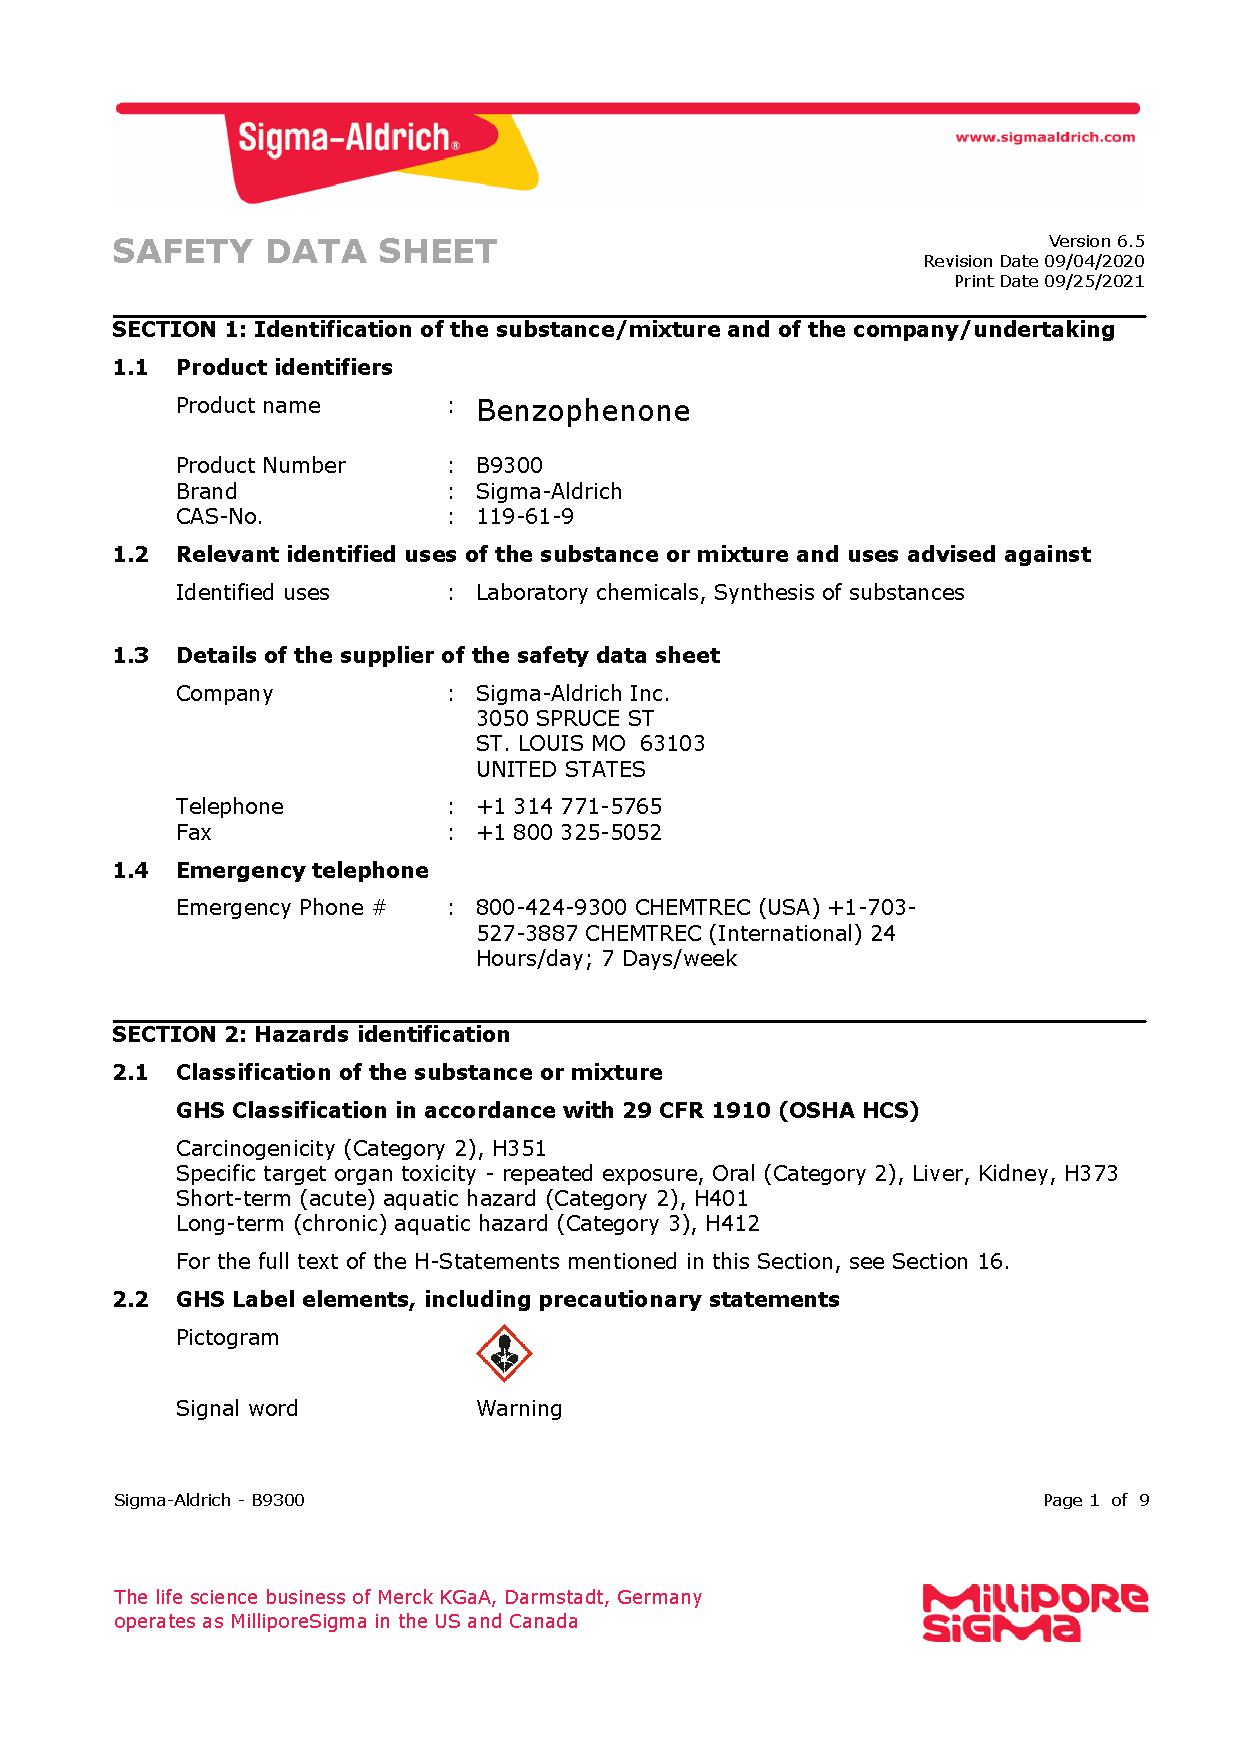
\includepdf[pages=-]{../../ExtFiles/BenzophenoneSDS-SA.pdf}
    \item ThermoFischer Scientific:
    \begin{itemize}
        \item Carcinogenicity (Category 2) --- serious.
        \item Combustible dusts (Category 1) --- severe.
        \item Oral ($\text{LD}_{50}$): $>\SI[per-mode=symbol]{10}{\gram\per\kilo\gram}$.
        \item Inhalation ($\text{Lc}_{50}$): N/a.
    \end{itemize}
    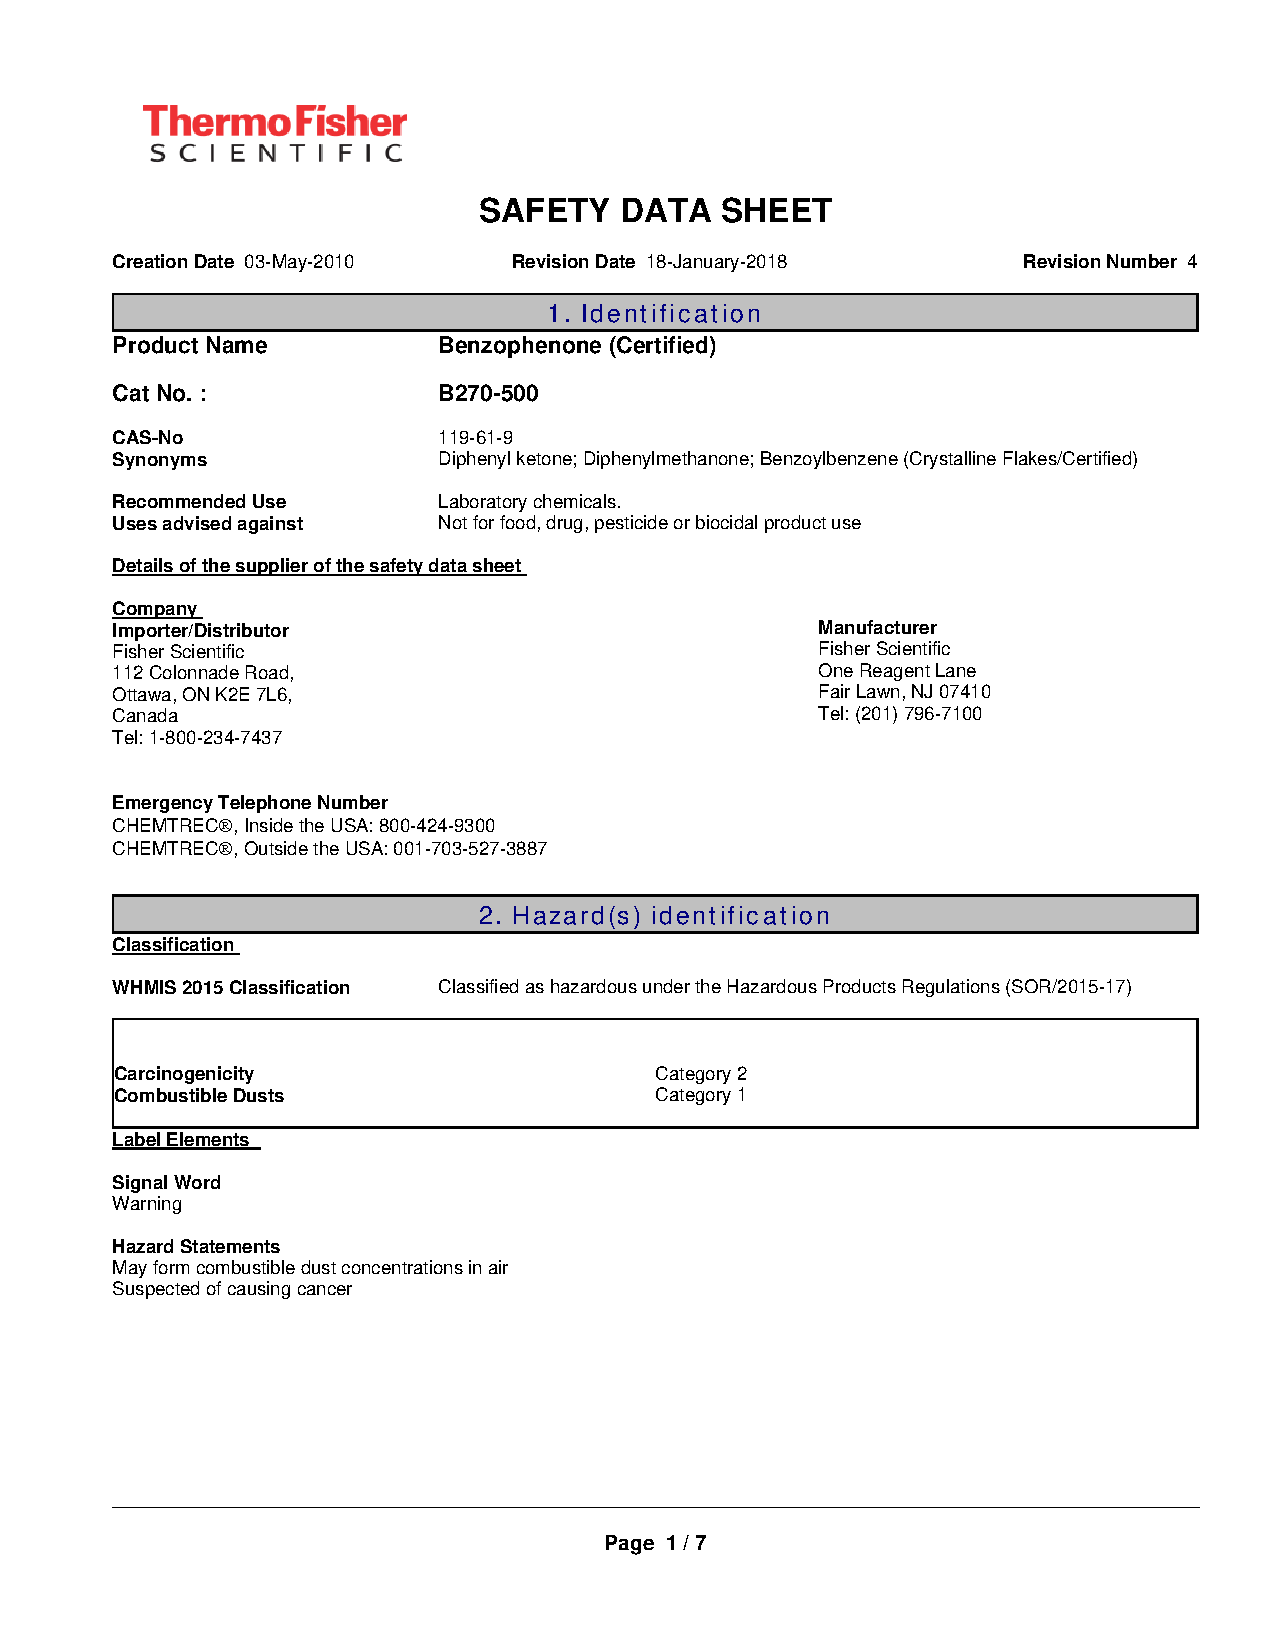
\includepdf[pages=-]{../../ExtFiles/BenzophenoneSDS-FS.pdf}
    \item The only category 1 hazard listed on either SDS was combustible dusts, so that is likely the most severe hazard.
\end{enumerate}
\newpage



\printbibliography




\end{document}